\begin{figure}[t]
    \centering
    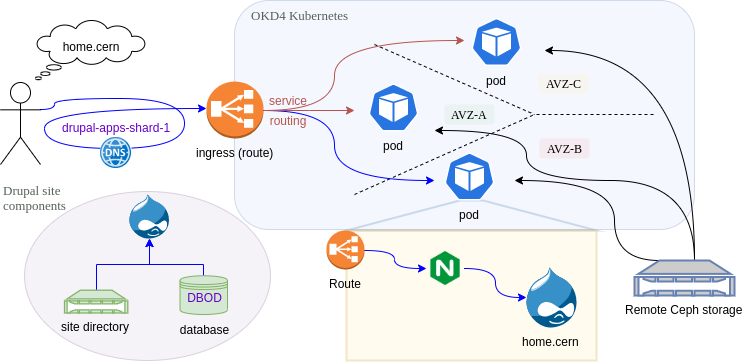
\includegraphics[width=\textwidth]{figures/drupal-k8s-request-journey}
    \caption{\emph{Request journey in the Kubernetes infrastructure}. Contrast with figure \ref{fig:drupal-physical-request-journey}.}
    \label{fig:drupal-k8s-request-journey}
\end{figure}

\subsection{Common Kubernetes infrastructure for all Web Frameworks}
\label{sec-web-frameworks}

\begin{table}[h!]
\begin{tabularx}{\textwidth}{ p{10em}| >{\raggedright\arraybackslash}X}
    \emph{Name} & \emph{Indicative use case} \\
    \hline \\
    EOS web hosting & Serve static HTML/CSS/JS/CGI stored on the EOS shared filesystem with simple deployment requirements \\
    CMS/Drupal & \hyperref[what-is-drupal]{Content Management System} for visual content creation and public outreach \\
    Platform as a Service (PaaS) & Custom web applications with flexible deployment on Openshift (Kubernetes) \\
    Discourse & A home for communities around a common topic \\
    TWiki & Wiki format content creation platform
\end{tabularx}
\caption{\emph{Web Frameworks}: web hosting and content creation platforms based on different technologies.
EOS web hosting ("WebEOS") is already using the common Kubernetes infrastructure.}
\label{tab-wf}
\end{table}

For each web framework there is currently a separate infrastructure, based on different technologies.
This creates silos of operational expertise within the small engineering team that supports each one, which are \emph{costly and inefficient} to keep alive in CERN's dynamic working environment.
At the same time there are a lot of software components developed in-house to support a single use case at the time, generating a large technical debt.
Many requirements however are shared, such as interfacing with external CERN systems.

We therefore developed a common platform on the \emph{Openshift Kubernetes community distribution (OKD 4)},
leaving only a thin business logic layer specific to each use case.
OpenShift was chosen firstly for its production-tested multitenancy support, which we relied on for the present PaaS infrastructure.
Openshift extends Kubernetes with tooling that simplifies our design \cite{jarvinen_extending_2019}:
a developer-focused console UI that we expose to end users, in-place upgrades of the control plane, node (machine) management API, monitoring and logging stacks.

The first web framework to use the new infrastructure is EOS web hosting ("WebEOS"), which has been \emph{in production since November 2020}.
At the same time, the Platform as a Service and Drupal use cases are in Pilot phase, due to enter production in 2021.

\subsection{Drupal on Kubernetes}

\begin{figure}[t]
    \centering
    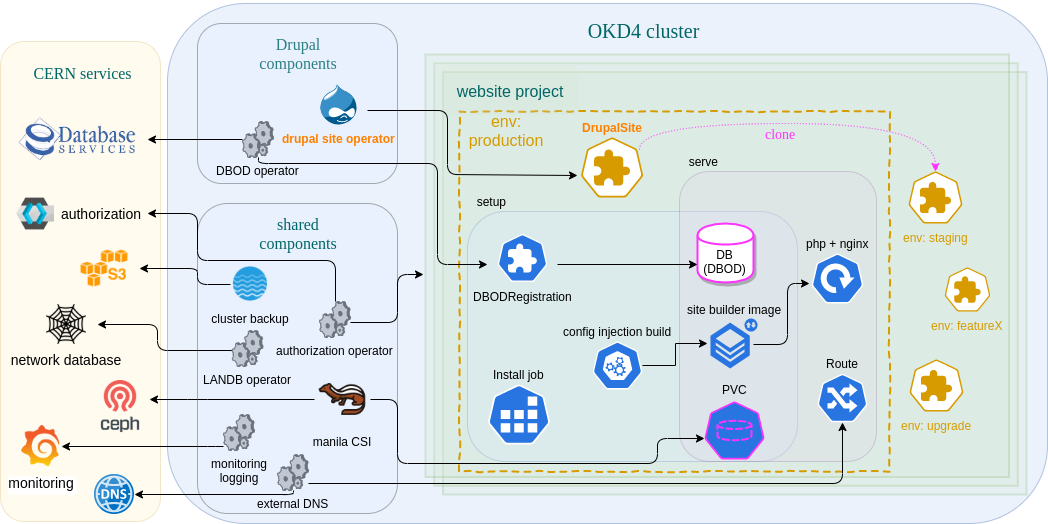
\includegraphics[width=1.05\textwidth]{figures/drupal-components}
    \caption{\emph{Drupal cluster architecture}.
    The diagram presents the Kubernetes resources that {\color{darkseagreen} make up a Drupal site},
    the {\color{carolinablue} controllers} that manage them and the cluster infrastructure,
    and the {\color{beige} external CERN systems} with which the cluster integrates.
    The Drupal API is the {\color{fluorescentorange} DrupalSite CRD}.}
    \label{fig:drupal-components}
\end{figure}

The physical servers are replaced with a cluster of virtual machines composing an OKD 4 cluster.
Each website is served by 1 or multiple replicas of a pod with Nginx and PHP-FPM containers.
The server perspective can be seen by following an HTTP request in figure \ref{fig:drupal-k8s-request-journey},

The infrastructure can be seen as an application that offers its users functions to manage websites.
It provides an API for website admins to specify the kind of website they need: what version of Drupal, what amount of resources, which git repository to fetch configuration from.
Website admins can similarly create different \emph{environments} of their website for development or test purposes,
clone data between websites, and take and restore backups.
An overview of the components is in figure \ref{fig:drupal-components}.

\subsubsection{Components}

We can define 3 component layers on top of Kubernetes:
\begin{enumerate}
    \item OpenShift
    \item Shared components: integration with CERN services, DNS, Network and Monitoring, cluster backups.
    \item Business logic: website management APIs and automation of operations
\end{enumerate}

Following the operator pattern introduced in section \ref{sec-operators}, the business logic (DrupalSite API) is implemented with the DrupalSite Custom Resource Definition (CRD) and the drupalSite operator.
Each website runs an immutable version of Drupal code
% TODO

TODO
- environments
- config injection
- clone




%%% NOTES %%%

%diagrams
%- admin workflow to update Drupal version

\subsubsection*{Website management functions}


CMS-based websites are inherently stateful applications: end users interact with them constantly and progress their state,
which is stored in a database and in a persistent volume.
To facilitate development, the state of a Drupal application can be "cloned" into another Drupal website.
The development workflow includes ... % TODO

% - L7 cloud load balancing for .cern domains?